\chapter{Versuchsdurchführung}
Das Ziel dieses Versuchs war es drei Grüßen zu bestimmen, die Frequenz des Lasers, den Brechungsindex von Luft, sowie den Brechungsindex eines Glasplättchens. Dazu wurden drei verschieden Versuchsschemen implementiert. Jeder dieser Varianten verwendet den allgemeinen Aufbau eines Michelson Interferometers (\figref{fig:aufbau})\\\\
Im ersten Teil, zur Bestimmung der Wellenlänge des Lasers, befindet sich keine Probe im Strahlengang. Die einzige Ursache der optischen Wegdifferenz ist Position der Spiegel. Gemäß \eqref{eq:phasendiff_ebenen} ändert sich die Phasendifferenz mit diesem Abstand. Betrachten wir das Zentrum des Interferenzmusters ist $\alpha=0$. Wenn wir nun, unter kontinuierlicher Änderung des Abstands $d$, zählen wie oft sich im Interferenzzentrum ein Intensitätsmaximum befindet, das sich dann mit sich änderndem $d$ nach außen bewegt, können wir die Wellenlänge des Lasers abschätzen. Es gilt nach \eqref{eq:phasendiff_ebenen}
\begin{align*}
    n=\frac{d}{\lambda}
\end{align*}

Im zweiten Teil des Versuchs soll der Brechungsindex eines Glasplättchens bestimmt werden. 
\begin{figure}[H]\label{fig:beugung_glas}
    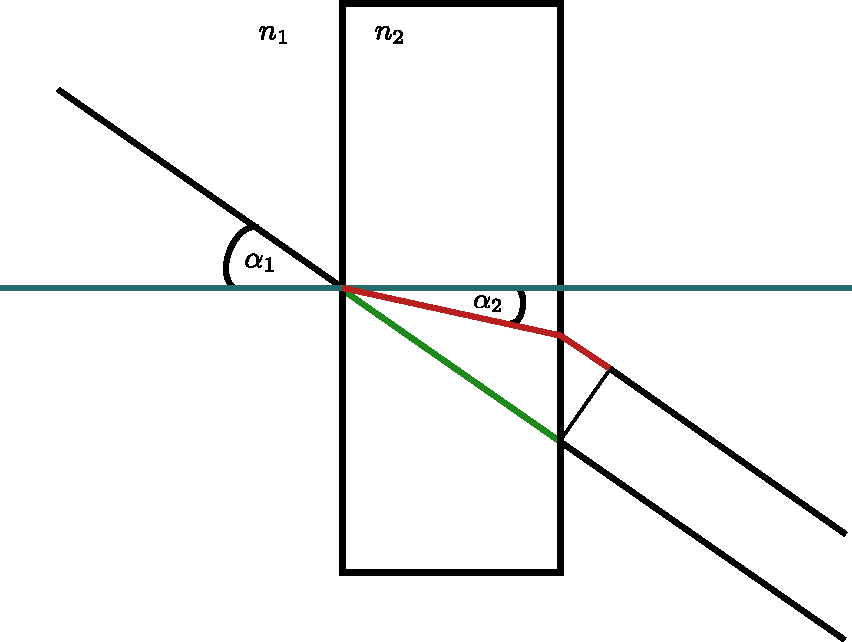
\includegraphics[scale=0.7]{pictures/path7.pdf}\label{fig:aufbau}
    \caption{\textbf{Wegunterschied bei Strahlengang durch Glasplättchen.} Das Glasplättchen wird durch das schwarze Rechteck dargestellt. Der Brechungsindex innerhalb ist mit $n_2$ gelabelt, außerhalb mit $n_1$. Ein Lichtstrahl, der unter dem Winkel $\alpha_1$ auf das Glasplättchen trifft, wird aufgrund des höheren Brechungsindex in Glas zum Lot hin gebrochen. Die rote Linie zeigt den Weg durch das Glas. Grün gibt als Referenz den Strahlengang an, wenn kein Glasplättchen da ist.}
\end{figure}
Wie in \figref{fig:beugung_glas} gezeigt, vergrößert sich der optische Weg, wenn der Strahl durch ein Glasplättchen fällt, das unter dem Winkel $\alpha_1$ in den Weg des Lichts eingeführt wird. $\alpha_1$ ist hier $0°$, wenn das Licht senkrecht auf das Glas trifft. Bei einer Dicke $b$ des Plättchens, berechnet sich der optische Weg durch das Glas $\text{OP}_1$ (rot) als
\begin{align*}
    \text{OP}_1=\frac{n_2b}{\cos\alpha_2}+\sin\alpha_1\,b\,n_1\,\left( \tan\alpha_1-\tan\alpha_2 \right)
\end{align*}
Der optische Weg ohne vorhandenes Glasplättchen ergibt sich entsprechend als
\begin{align*}
    \text{OP}_2=\frac{n_1b}{\cos\alpha_1}
\end{align*}
Folglich stellt sich eine Wegdifferenz ein von
\begin{align*}
    \text{OP}_1-\text{OP}_2&=n_1b\,\frac{\sin^2\alpha_1-1}{\cos\alpha_1}+b\,\frac{n_2-n_1\sin\alpha_1\sin\alpha_2}{\cos\alpha_2}
\end{align*}
Gemäß des Snelliusschen Brechungsgesetzes vereinfacht sich dies zu
\begin{align}
    \text{OP}_1-\text{OP}_2&=n_1b\,\frac{\sin^2\alpha_1-1}{\cos\alpha_1}+b\,\frac{n_2-n_2\sin^2\alpha_2}{\cos\alpha_2}\notag\\
    &=n_2b\,\cos\alpha_2-n_1b\,\cos\alpha_1\notag\\
    &=n_2b\,\sqrt{1-(\frac{n_1}{n_2}\,\sin\alpha_1)^2}-n_1b\,\cos\alpha_1
\end{align}%\label{eq:deltaR_glas}
Diese Gleichung gilt für den Strahl, der das Zentrum des Interferenzmusters trifft, und bleibt eine gute Näherung, wenn man sich nicht weit davon entfernt. Im Versuch wird mittels einer Photodiode die Intensität an einer Stelle auf dem Schirm gemessen. Wenn nun der Winkel, unter dem das Glasplättchen in den Strahlengang eingeführt wird, verändert wird, ändert sich die Intensität. Mit Hilfe von Cassy werden gleichzeitig Winkel und Intensität gemessen. Über eine Anpassung des Intensitätsverlaufs an den theoretischen Zusammenhang aus %\eqref{eq:deltaR_glas} 
kann sowohl die Dicke als auch der Brechungsindex des Plättchens bestimmt werden.\\\\

Als dritten Teil des Versuchs sollte der Brechungsindex von Luft berechnet werden. Dazu wird eine Gaszelle der Länge $10\pm0.1\,$cm in einen der Strahlengänge eingebracht. Der Druck $p$ in der Gaszelle wird durch eine Vakuumpumpe gesteuert. Der Wegunterschied ergibt sich analog zum vorherigen Aufbau mit dem Glasplättchen, unter Berücksichtigung, dass die Gaszelle horizontal in den Strahlengang geführt wird. Daraus ergibt sich ein optischer Wegunterschied von
\begin{align*}
    \Delta \text{OP}&=(n_2(p)-n_1)\,b
\end{align*}
Da im Praktikum keine Zeit war diesen Versuch durchzuführen, erhielten wir Messdaten von unserem Betreuer. Es wird erwartet, dass sich der Brechungsindex linear mit dem Druck ändert. Dies muss im Experiment überprüft werden. Durch Extrapolation kann dann der Brechungsindex bei normal Druck ermittelt werden.